\section{Theoretical Analysis}
\label{sec:analysis}

The transformer with a n:1 ratio was used, which means that the initial voltage will have its amplitude (230 V) multiplied by a factor n. This way, the voltage at the terminals of the transformer can be represented as a voltage source with an amplitude of $230n$ but with the same frequency as the initial source.

\subsection{Step 1: Solution for the Envelope Detector}

The output of the transformer will be the input of the Envelope detector, which is made of a rectifier and a capacitor. The rectifier is a full-wave bridge rectifier circuit  and is composed of 4 diodes and a resistor, as shown:

\begin{figure}[h] \centering
\includegraphics[height=6cm]{Circuit_envelope.pdf}
\caption{Envelope Detector circuit.}
\label{fig:ENV_CIR}
\end{figure}

In this case, we have chosen to aproximate the diodes to the ideal model + $V_{on}$, in which $V_{on} = 0.70V$. Knowing also that only one way is used when the diodes are on, we can further simplify the circuit as shown in Figure~\ref{fig:ENV_CIR_S}. We can also say that $V_{in}(t) = V_s(t) - 2V_{on}, V_s(t) - 2V_{on} > 0$ or $V_{in}(t) = 0, V_s(t) - 2V_{on} < 0$.

\begin{figure}[h] \centering
\includegraphics[height=6cm]{Circuit_envelope_simple.pdf}
\caption{Envelope Detector circuit simplified, when the diodes are on.}
\label{fig:ENV_CIR_S}
\end{figure}

Using the full-wave rectifier instead of the half-wave enables the decrease of the ripple withoud increasing the time constant, reducing the costs. This is possible because the voltage that comes out of the transformer will leave the rectifier oscillating at twice the frequency, which reduces the period corresponding to the wave ripple.

To compute the voltage in the capacitor we need to take in account the possibility of the diodes being turned off. This will happen when $V_C > V_{in}$, and, in this case the voltage in the capacitor will decay as:
\begin{equation}
  V_{C}(t) = Ae^{-\frac{t}{RC}},
  \label{eq:vc_nat}
\end{equation}
where $A$ is the voltage right before the diodes are turned off.
When the diodes are on, $V_C = V_{in}$.
As such, we have to calculate when the diodes are turned off and on. To estimate the first we have noticed that the discharge of the capacitor is limited by equation~\ref{eq:vc_nat}. In other words, knowing that in the moment before being turned off, $V_C = V_{in}$, we just have to evaluate

\begin{equation}
  V_{C}(t) = V_{in}(t-\delta) e^{-\frac{\delta}{RC}} > V_{in}(t).
  \label{eq:vc_off}
\end{equation}

where we assume that the diodes have been turned off.If the expression is true, then the voltage in the diodes becomes negative, what means that it is turned off and voltage in the capacitor decays as described in equation~\ref{eq:vc_nat}. If the expression is false, the voltage in the diodes stays positive, and the diodes stay on.
To know when the diodes are turned on again, we just have to know when $V_{c}(t)<V_{in}(t)$. From that point on, the diodes are turned on, until the innequality \ref{eq:vc_off} is valid again.

The result of this analisys is the following:

\begin{figure}[h] \centering
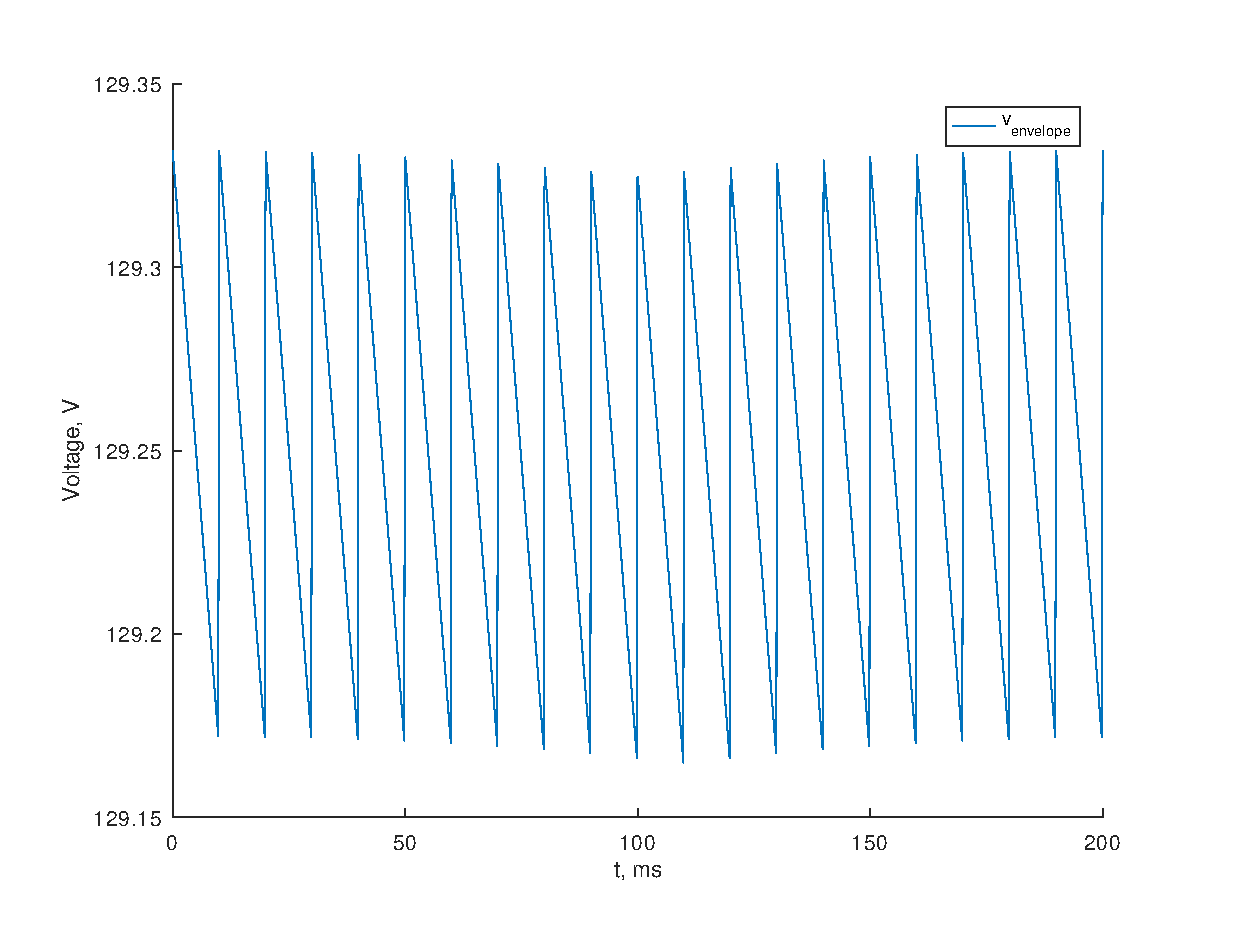
\includegraphics[height=8cm]{PASSO41.eps}
\caption{Envelope detector $V_{envelope}$.}
\label{fig:TEO_ENV}
\end{figure}

\newpage

\subsection{Step 2: Solution for the Voltage Regulator}

Then, the output of the Envelope Detector is the input of the Voltage Regulator. The last one is made of a resistor and diodes in series. Its output is the voltage in the diodes, as represented:

\begin{figure}[h] \centering
\includegraphics[height=6cm]{Circuit_regulator.pdf}
\caption{Voltage Regulator.}
\label{fig:TEO_VR_CIR}
\end{figure}

In the Envolope Detector the diode model used has an ideal diode and a voltage source while in the Voltage Regulator the diode model (where we have said that the emition coefition is $\eta m$, being $m=18$ the number of diodes in the regulator) has an ideal diode, a voltage source, $V_{d}$ and a resistor $r_{d}$. 

\begin{figure}[h] \centering
\includegraphics[height=6cm]{Circuit_regulator_simple.pdf}
\caption{Simplification of the Voltage Regulator.}
\label{fig:TEO_VR_CIR_S}
\end{figure}

The steps to know each one of this constants are described in the theory classes:
$V_{d}$ is determined by solving the non linear equation

\begin{equation}
  V_d + R*Is*(exp(V_d/(V_Tm))-1) = V_c.
  \label{eq:Vd}
\end{equation}

$r_{d}$ is then calculated with the folowing expression:

\begin{equation}
  r_{d} = V_T*n/( Is*(exp(V_d/(V_Tm)))).
  \label{eq:Rd}
\end{equation}

From here we say that

\begin{equation}
  V_{D} = V_d + ir_d; \text{ where } i = \frac{V_C-V_d})/(R_2+r_d);
  \label{eq:TEO_VD}
\end{equation}

Or, in words, $i$ is the current passing through the diode because of the non constant voltage.

The plots for $V_{out}$, $V_{out} - 12V$ and the pair $V_c$, $V_{out}$ are the following:

\begin{figure}[h] \centering
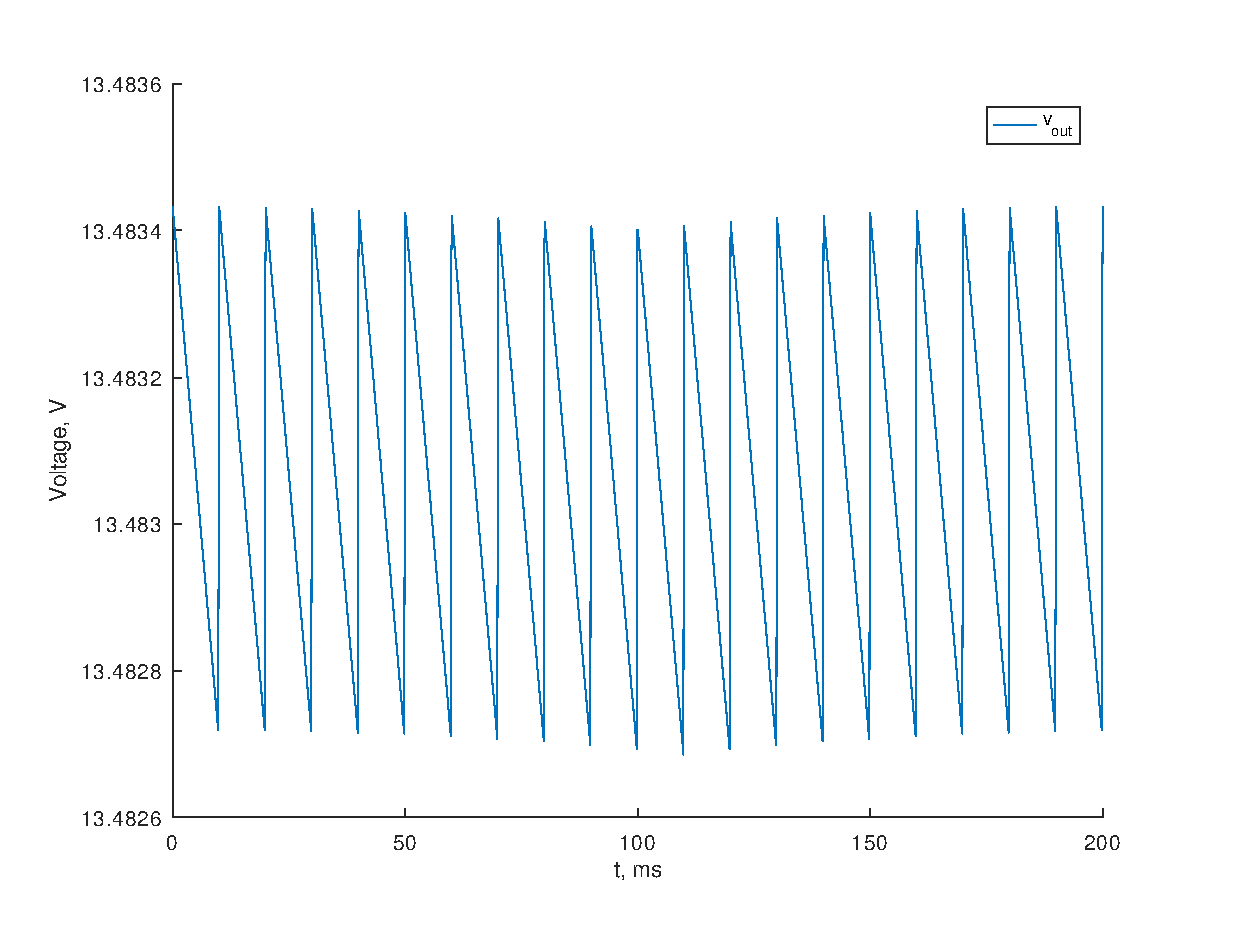
\includegraphics[height=8cm]{PASSO42.eps}
\caption{$V_{out}$.}
\label{fig:TEO_OUT}
\end{figure}

\begin{figure}[h] \centering
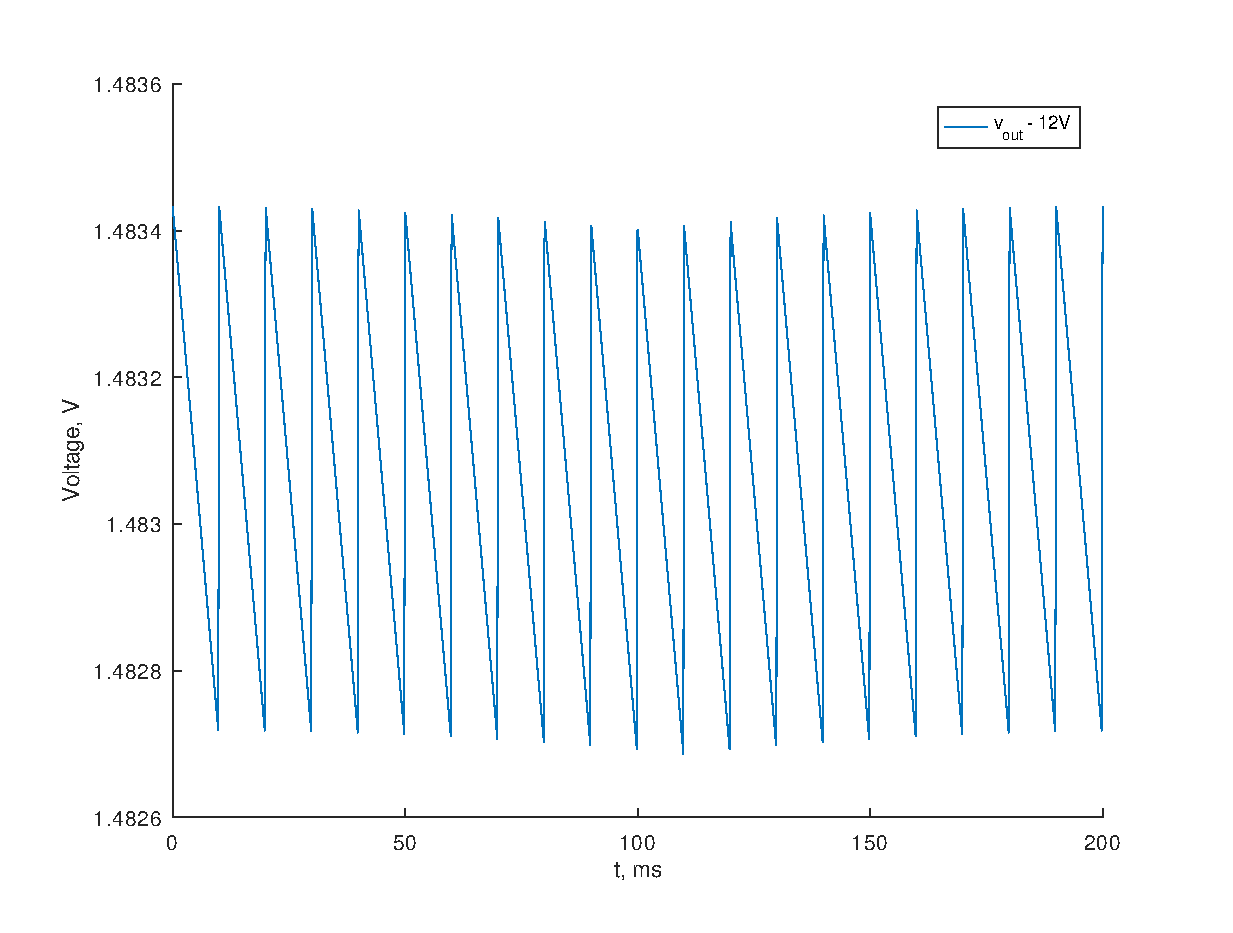
\includegraphics[height=8cm]{PASSO5.eps}
\caption{$V_{out} - 12V$.}
\label{fig:TEO_OUT-12}
\end{figure}

\newpage

\begin{figure}[h] \centering
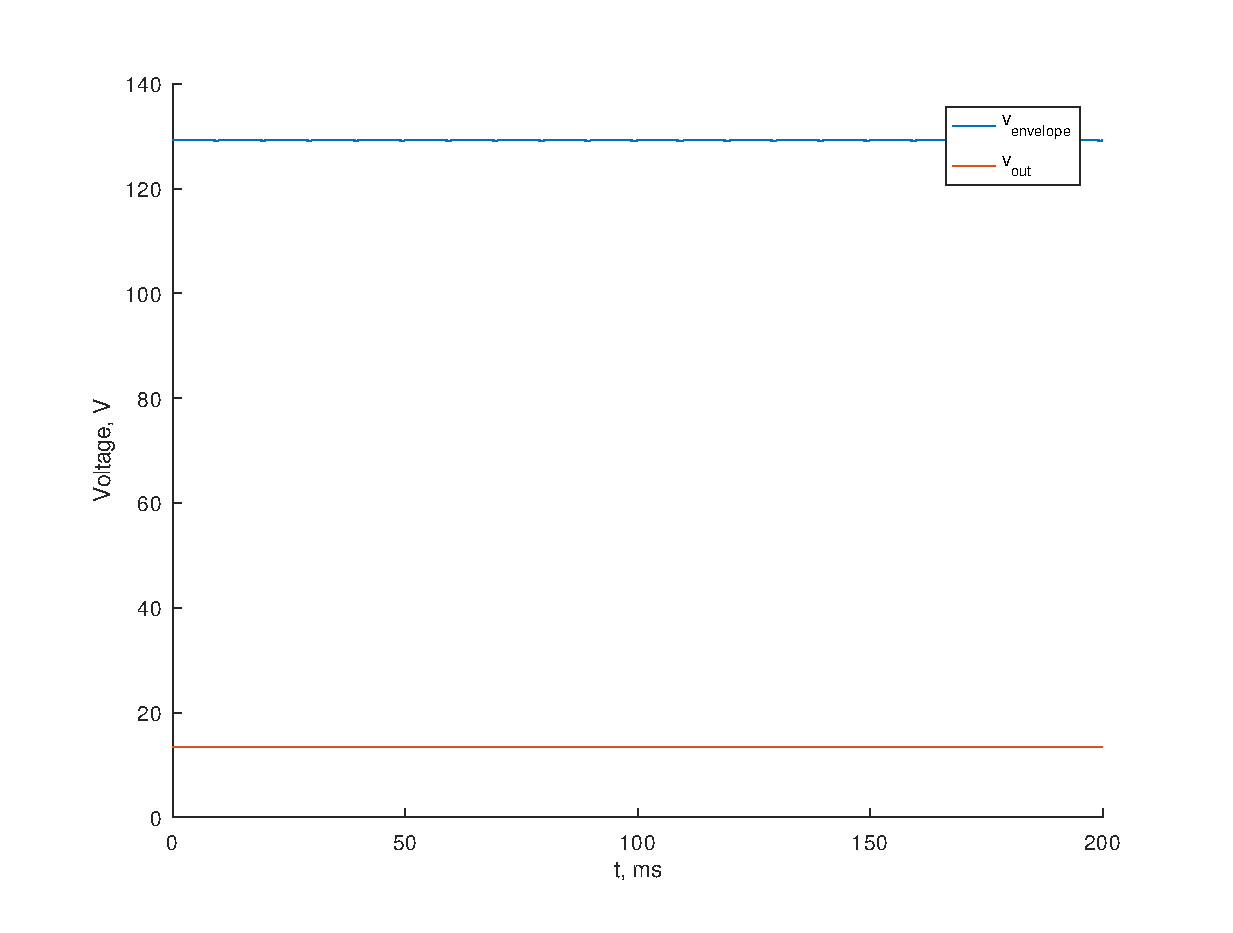
\includegraphics[height=8cm]{PASSO4.eps}
\caption{$V_c$ and $V_{out}$.}
\label{fig:TEO_FULL}
\end{figure}

The results from the theoretical analysis are the following:

\begin{table}[h]
  \centering
  \begin{tabular}{|l|r|}
    \hline    
    {\bf Name} & {\bf Value} \\ \hline
    \input{../mat/MAT_tab}
  \end{tabular}
  \caption{Variables are of type {\em voltage} and expressed in Volt.}
  \label{tab:TEO_RES}
\end{table}